%===============================================================================
% LaTeX sjabloon voor de bachelorproef toegepaste informatica aan HOGENT
% Meer info op https://github.com/HoGentTIN/latex-hogent-report
%===============================================================================

\documentclass[dutch,dit,thesis]{hogentreport}

\usepackage{lipsum} % For blind text, can be removed after adding actual content

%% Pictures to include in the text can be put in the graphics/ folder
\graphicspath{{../graphics/}}

%% For source code highlighting, requires pygments to be installed
%% Compile with the -shell-escape flag!
%% \usepackage[chapter]{minted}
%% If you compile with the make_thesis.{bat,sh} script, use the following
%% import instead:
\usepackage[chapter,outputdir=../output]{minted}
\usemintedstyle{solarized-light}

%% Formatting for minted environments.
\setminted{%
    autogobble,
    frame=lines,
    breaklines,
    linenos,
    tabsize=4
}

%% Ensure the list of listings is in the table of contents
\renewcommand\listoflistingscaption{%
    \IfLanguageName{dutch}{Lijst van codefragmenten}{List of listings}
}
\renewcommand\listingscaption{%
    \IfLanguageName{dutch}{Codefragment}{Listing}
}
\renewcommand*\listoflistings{%
    \cleardoublepage\phantomsection\addcontentsline{toc}{chapter}{\listoflistingscaption}%
    \listof{listing}{\listoflistingscaption}%
}

% Other packages not already included can be imported here
\usepackage{pgfplots}
\pgfplotsset{compat=1.18}
\usepackage{pgfplotstable}

%%---------- Document metadata -------------------------------------------------
% TODO: Replace this with your own information
\author{Dhondt Milan}
\supervisor{Mevr. V. Depestele}
\cosupervisor{Dhr. T. Aelbrecht}
\title
    {De bruikbaarheid en betrouwbaarheid van LLM gegenereerde feedback op studentenprojecten binnen Front-end Web Development en Web Services.}
\academicyear{\advance\year by -1 \the\year--\advance\year by 1 \the\year}
\examperiod{1}
\degreesought{\IfLanguageName{dutch}{Professionele bachelor in de toegepaste informatica}{Bachelor of applied computer science}}
\partialthesis{false}
%\institution{Internshipcompany BVBA.}

%% Add global exceptions to the hyphenation here
\hyphenation{back-slash}

%% The bibliography (style and settings are  found in hogentthesis.cls)
\addbibresource{bachproef.bib}            %% Bibliography file
\addbibresource{../voorstel/voorstel.bib} %% Bibliography research proposal
\defbibheading{bibempty}{}

%% Prevent empty pages for right-handed chapter starts in twoside mode
\renewcommand{\cleardoublepage}{\clearpage}

\renewcommand{\arraystretch}{1.2}

%% Content starts here.
\begin{document}

%---------- Front matter -------------------------------------------------------

\frontmatter

\hypersetup{pageanchor=false} %% Disable page numbering references
%% Render a Dutch outer title page if the main language is English
\IfLanguageName{english}{%
    %% If necessary, information can be changed here
    \degreesought{Professionele Bachelor toegepaste informatica}%
    \begin{otherlanguage}{dutch}%
       \maketitle%
    \end{otherlanguage}%
}{}

%% Generates title page content
\maketitle
\hypersetup{pageanchor=true}

%%=============================================================================
%% Voorwoord
%%=============================================================================

\chapter*{\IfLanguageName{dutch}{Woord vooraf}{Preface}}
\label{ch:voorwoord}

Het schrijven van deze bachelorproef vormt het sluitstuk van mijn opleiding Toegepaste Informatica aan HOGENT. Hoewel mijn opleiding als Full Stack Developer zich voornamelijk richt op het ontwikkelen van software, heb ik bewust gekozen voor een onderwerp rond artificiële intelligentie. De snelle opkomst van AI en de steeds grotere impact ervan op softwareontwikkeling maakten dit voor mij een bijzonder interessante en relevante piste om verder te verkennen.

\vspace{1em}

In deze bachelorproef werd onderzocht in welke mate Large Language Models (LLM’s) bruikbare en betrouwbare feedback kunnen genereren op de codekwaliteit van studentenprojecten binnen de opleidingsonderdelen Front-end Web Development en Web Services. Dit onderzoek vertrekt vanuit een concreet probleem, waarbij de evaluatie van projecten tijdsintensief is en onderhevig kan zijn aan inconsistenties. Door middel van een literatuurstudie, interviews met lectoren en de ontwikkeling van een proof-of-concept werd nagegaan hoe LLM’s hierin een ondersteunende rol kunnen spelen.

\vspace{1em}

Het uitvoeren van dit onderzoek was een leerrijk proces waarin ik niet alleen mijn technische vaardigheden verder heb ontwikkeld, maar ook kritisch heb leren nadenken over de rol van AI binnen het programmeeronderwijs. Het bood mij de kans om mijn interesse in softwareontwikkeling te combineren met de mogelijkheden van nieuwe technologieën.

\vspace{1em}

Graag wil ik een aantal personen bedanken die hebben bijgedragen aan deze bachelorproef. In de eerste plaats wil ik mijn promotor, Mevr. V. Depestele, bedanken voor de begeleiding, de waardevolle feedback en de ondersteuning doorheen het volledige traject. Daarnaast wil ik mijn co-promotor, Dhr. T. Aelbrecht, bedanken voor het meedenken en de technische inzichten die hebben bijgedragen aan dit onderzoek. Verder wil ik ook de lector(en) bedanken die hebben meegewerkt aan het onderzoek en hun inzichten hebben gedeeld over het evaluatieproces van studentenprojecten. Hun input was van grote waarde voor de uitwerking van deze bachelorproef.

\vspace{1em}

Tot slot wil ik mijn familie en vrienden bedanken voor hun blijvende steun en aanmoediging tijdens mijn opleiding. Met deze bachelorproef hoop ik een bijdrage te leveren aan het inzicht in de mogelijkheden en beperkingen van LLM’s binnen het programmeeronderwijs, en een basis te bieden voor verder onderzoek naar de integratie van AI in evaluatieprocessen.

%%=============================================================================
%% Samenvatting
%%=============================================================================

% TODO: De "abstract" of samenvatting is een kernachtige (~ 1 blz. voor een
% thesis) synthese van het document.
%
% Een goede abstract biedt een kernachtig antwoord op volgende vragen:
%
% 1. Waarover gaat de bachelorproef?
% 2. Waarom heb je er over geschreven?
% 3. Hoe heb je het onderzoek uitgevoerd?
% 4. Wat waren de resultaten? Wat blijkt uit je onderzoek?
% 5. Wat betekenen je resultaten? Wat is de relevantie voor het werkveld?
%
% Daarom bestaat een abstract uit volgende componenten:
%
% - inleiding + kaderen thema
% - probleemstelling
% - (centrale) onderzoeksvraag
% - onderzoeksdoelstelling
% - methodologie
% - resultaten (beperk tot de belangrijkste, relevant voor de onderzoeksvraag)
% - conclusies, aanbevelingen, beperkingen
%
% LET OP! Een samenvatting is GEEN voorwoord!

\chapter*{\IfLanguageName{dutch}{Samenvatting}{Abstract}}

Large Language Models (LLM's) worden niet alleen steeds beter in het schrijven van code, maar ook in het nakijken en analyseren ervan. Binnen het programmeeronderwijs, zoals bij de opleidingsonderdelen Front-End Web Development en Web Services aan HOGENT, kruipt er elk jaar enorm veel tijd in het evalueren van studentenprojecten. Lectoren moeten tientallen criteria handmatig aftoetsen per ingediend project. Dat nakijkwerk is niet alleen tijdrovend en repetitief, maar laat soms ook ruimte voor inconsistenties, waardoor er minder tijd overblijft om echt diepgaande en nuttige feedback te schrijven voor de student.

\vspace{1em}

Deze bachelorproef onderzoekt de inzet van LLM's als geautomatiseerde 'assistent-evaluatoren'. De centrale vraag is: in welke mate kunnen LLM's betrouwbare, objectieve en bruikbare feedback genereren op de code van studenten, en hoe verhoudt dit oordeel zich tot dat van de menselijke docenten?

\vspace{1em}

Om dit in de praktijk te testen, werd er een \textit{proof-of-concept} (PoC) ontwikkeld. Binnen een veilige, geïsoleerde cloud-omgeving (een E2B sandbox) gaat een AI-pipeline iteratief door de code, documentatie en structuur van ingediende projecten. Hierbij werd gebruikgemaakt van Mastra AI en het krachtige \texttt{qwen3-coder:480b-cloud} model om acht projecten door te lichten op tientallen criteria. De resulterende JSON-rapporten van de AI werden vervolgens zowel kwantitatief als kwalitatief vergeleken met de originele evaluatiekaarten van de lectoren.

\vspace{1em}

De resultaten zijn veelbelovend. Bij de ontvankelijkheidscriteria, zoals het gebruik van een specifiek framework, formuliervalidatie of de aanwezigheid van testen, kwamen de resultaten in maar liefst 91,1\% van de gevallen overeen met het oordeel van de lector. Het LLM bleek ijzersterk in het opleveren van opvallend constructieve feedback, compleet met traceerbare verwijzingen naar specifieke bestandslocaties en lijnen code. Voor de meer complexe, kwalitatieve beoordelingen ('hoe mooi of herbruikbaar is deze feature ingericht?') botste het systeem aanvankelijk op de limieten van een "ja/nee"-schaal. Dit werd gelukkig met succes opgevangen door een rubric-beoordelingsstructuur te verwerken waarbij de AI het project automatisch afweegt tegen de voorbeeldapplicatie. 

\vspace{1em}

Natuurlijk zijn er nog beperkingen. Zo analyseert dit systeem de code vooral statisch en merkt het niet direct dat een app bij het lokaal opstarten meteen crasht (\textit{runtime} fouten). Ook neemt het sterke redeneerproces (\textit{thinking}) van dit specifieke AI-model nog een 8 tot 15 minuten analysetijd per project in beslag.

\vspace{1em}

Kortom, de inzet van LLM-gebaseerde evaluatietools luidt een efficiëntere toekomst in voor het programmeeronderwijs. Hoewel AI de menselijke beoordelaar (nog) niet volledig vervangt, bewijst dit onderzoek wel luid en duidelijk dat het de zware nakijklast drastisch kan verlichten door in te springen als een betrouwbare en objectieve controleur.


%---------- Inhoud, lijst figuren, ... -----------------------------------------

\tableofcontents

% In a list of figures, the complete caption will be included. To prevent this,
% ALWAYS add a short description in the caption!
%
%  \caption[short description]{elaborate description}
%
% If you do, only the short description will be used in the list of figures

\listoffigures

\begin{figure}[htbp]
    \centering
    \begin{tikzpicture}
        \begin{axis}[
            ybar,
            width=0.9\textwidth,
            height=7cm,
            ylabel={Nauwkeurigheid (\%)},
            symbolic x coords={P-01,P-02,P-03,P-04,P-05,P-06,P-07,P-08},
            xtick=data,
            xlabel={Project},
            ymin=0, ymax=110,
            ytick={0,20,40,60,80,100},
            bar width=18pt,
            nodes near coords,
            nodes near coords align={vertical},
            every node near coord/.append style={font=\small\bfseries},
            enlarge x limits=0.12,
            grid=major,
            grid style={dashed,gray!30},
            fill=blue!60,
            ]
            \addplot coordinates {
                (P-01, 100)
                (P-02, 90)
                (P-03, 100)
                (P-04, 90)
                (P-05, 90)
                (P-06, 60)
                (P-07, 100)
                (P-08, 100)
            };
        \end{axis}
    \end{tikzpicture}
    \caption[Nauwkeurigheid ontvankelijkheid per project]{Nauwkeurigheid van de AI-ontvankelijkheidsbeoordeling per project.}
    \label{fig:ontv-per-project}
\end{figure}

% If you included tables and/or source code listings, uncomment the appropriate
% lines.
\listoftables

\clearpage

\begin{table}[htbp]
    \centering
    \caption[Globale ontvankelijkheidsresultaten]{Globale vergelijking AI versus lector op de ontvankelijkheidscriteria.}
    \label{tab:ontv-globaal}
    \begin{tabular}{l r}
        \hline
        \textbf{Metriek} & \textbf{Waarde} \\
        \hline
        Totaal beoordeeld door AI & 87 \\
        Effectief gekoppeld aan lector & 79 \\
        Overeenkomsten (match) & 72 \\
        Afwijkingen (mismatch) & 7 \\
        \textbf{Nauwkeurigheid} & \textbf{91,1\%} \\
        \hline
    \end{tabular}
\end{table}

\begin{table}[htbp]
    \centering
    \caption[Overzicht geëvalueerde projecten]{Samenvatting van de geanalyseerde dataset per project en per flow. ``Aanw.'' = aanwezig, ``Afw.'' = afwezig, ``Ond.'' = onduidelijk.}
    \label{tab:dataset-overzicht}
    \small
    \begin{tabular}{l c c c c c c c}
        \hline
        \textbf{Project} & \multicolumn{3}{c}{\textbf{Ontvankelijkheid}} & \multicolumn{3}{c}{\textbf{Evaluatiecriteria}} & \textbf{Niet gecl.} \\
        & Aanw. & Afw. & Ond. & Aanw. & Afw. & Ond. & \\
        \hline
        fews-project-01 & 11 & 0 & 0 & 12 & 1 & 5 & 1 \\
        fews-project-02 & 10 & 1 & 0 & 16 & 3 & 0 & 0 \\
        fews-project-03 & 11 & 0 & 0 & 17 & 2 & 0 & 0 \\
        fews-project-04 & 10 & 1 & 0 & 16 & 3 & 0 & 0 \\
        fews-project-05 & 10 & 1 & 0 & 10 & 3 & 0 & 6 \\
        fews-project-06 & 6  & 5 & 0 & 11 & 8 & 0 & 0 \\
        fews-project-07 & 11 & 0 & 0 & 18 & 1 & 0 & 0 \\
        fews-project-08 & 10 & 0 & 1 & 18 & 1 & 0 & 1 \\
        \hline
    \end{tabular}
\end{table}

\clearpage

\begin{table}[htbp]
    \centering
    \caption[Ontvankelijkheid per project]{Detail per project: aantal overeenkomsten, afwijkingen en ontbrekende koppelingen.}
    \label{tab:ontv-per-project}
    \begin{tabular}{l c c c c}
        \hline
        \textbf{Project} & \textbf{Match} & \textbf{Mismatch} & \textbf{Geen data} & \textbf{Nauwk.} \\
        \hline
        fews-project-01 & 10 & 0 & 1 & 100\% \\
        fews-project-02 & 9  & 1 & 1 & 90\% \\
        fews-project-03 & 10 & 0 & 1 & 100\% \\
        fews-project-04 & 9  & 1 & 1 & 90\% \\
        fews-project-05 & 9  & 1 & 1 & 90\% \\
        fews-project-06 & 6  & 4 & 1 & 60\% \\
        fews-project-07 & 10 & 0 & 1 & 100\% \\
        fews-project-08 & 9  & 0 & 1 & 100\% \\
        \hline
        \textbf{Totaal} & \textbf{72} & \textbf{7} & \textbf{8} & \textbf{91,1\%} \\
        \hline
    \end{tabular}
\end{table}

\begin{table}[htbp]
    \centering
    \caption[Evaluatiecriteria overzicht]{Overzicht evaluatiecriteria: AI-oordelen versus lector-scores per project.}
    \label{tab:eval-overview}
    \small
    \begin{tabular}{l c c c c c c}
        \hline
        \textbf{Project} & \multicolumn{3}{c}{\textbf{AI-oordeel}} & \multicolumn{2}{c}{\textbf{Lector-criteria met score}} \\
        & Aanw. & Afw. & Ond. & WS (gescoord) & FE (gescoord) \\
        \hline
        fews-project-01 & 12 & 1 & 5 & 32 & 26 \\
        fews-project-02 & 16 & 3 & 0 & 27 & 24 \\
        fews-project-03 & 17 & 2 & 0 & 32 & 27 \\
        fews-project-04 & 16 & 3 & 0 & 31 & 27 \\
        fews-project-05 & 10 & 3 & 0 & 25 & 26 \\
        fews-project-06 & 11 & 8 & 0 & 33 & 0 \\
        fews-project-07 & 18 & 1 & 0 & 32 & 27 \\
        fews-project-08 & 18 & 1 & 0 & 32 & 26 \\
        \hline
    \end{tabular}
\end{table}

\begin{table}[htbp]
    \centering
    \caption[Analyse afwezig-oordelen]{Criteria die de AI als ``afwezig'' beoordeelde, met het corresponderende lector-oordeel.}
    \label{tab:afwezig-analyse}
    \small
    \begin{tabular}{l l l l}
        \hline
        \textbf{Project} & \textbf{Criterium (AI)} & \textbf{Domein} & \textbf{Lector} \\
        \hline
        \multicolumn{4}{l}{\textit{Terugkerend over meerdere projecten}} \\
        Alle proj. & Anti-patterns React Hooks & FE & Niet apart \\
        Proj. 02, 03, 04 & Isolatie datalaag (geen SQL in services) & WS & Niet apart \\
        \hline
        \multicolumn{4}{l}{\textit{Projectspecifiek}} \\
        Proj. 02 & Foutafhandeling REST API & WS & C \\
        Proj. 04 & REST API CRUD-operaties & WS & C \\
        Proj. 05 & Formulier afhandeling & FE & Niet apart \\
        Proj. 05 & Client-side authenticatie & FE & Niet apart \\
        Proj. 06 & Minimale logging en configuratie & WS & C \\
        Proj. 08 & Anti-patterns React Hooks & FE & Niet apart \\
        \hline
    \end{tabular}
\end{table}

%---------- Kern ---------------------------------------------------------------

\mainmatter{}

% De eerste hoofdstukken van een bachelorproef zijn meestal een inleiding op
% het onderwerp, literatuurstudie en verantwoording methodologie.
% Aarzel niet om een meer beschrijvende titel aan deze hoofdstukken te geven of
% om bijvoorbeeld de inleiding en/of stand van zaken over meerdere hoofdstukken
% te verspreiden!

\input{inleiding}
\chapter{\IfLanguageName{dutch}{Stand van zaken}{State of the art}}%
\label{ch:stand-van-zaken}

% Tip: Begin elk hoofdstuk met een paragraaf inleiding die beschrijft hoe
% dit hoofdstuk past binnen het geheel van de bachelorproef. Geef in het
% bijzonder aan wat de link is met het vorige en volgende hoofdstuk.

% Pas na deze inleidende paragraaf komt de eerste sectiehoofding.

% ================================================================

% Dit hoofdstuk bevat je literatuurstudie. De inhoud gaat verder op de inleiding, maar zal het onderwerp van de bachelorproef *diepgaand* uitspitten. De bedoeling is dat de lezer na lezing van dit hoofdstuk helemaal op de hoogte is van de huidige stand van zaken (state-of-the-art) in het onderzoeksdomein. Iemand die niet vertrouwd is met het onderwerp, weet nu voldoende om de rest van het verhaal te kunnen volgen, zonder dat die er nog andere informatie moet over opzoeken.

% Je verwijst bij elke bewering die je doet, vakterm die je introduceert, enz.\ naar je bronnen. In \LaTeX{} kan dat met het commando \texttt{$\backslash${textcite\{\}}} of \texttt{$\backslash${autocite\{\}}}. Als argument van het commando geef je de ``sleutel'' van een ``record'' in een bibliografische databank in het Bib\LaTeX{}-formaat (een tekstbestand). Als je expliciet naar de auteur verwijst in de zin (narratieve referentie), gebruik je \texttt{$\backslash${}textcite\{\}}. Soms is de auteursnaam niet expliciet een onderdeel van de zin, dan gebruik je \texttt{$\backslash${}autocite\{\}} (referentie tussen haakjes). Dit gebruik je bv.~bij een citaat, of om in het bijschrift van een overgenomen afbeelding, broncode, tabel, enz. te verwijzen naar de bron. In de volgende paragraaf een voorbeeld van elk.

% Een schrijver schreef een van de standaardwerken over sorteer- en zoekalgoritmen. Experten zijn het erover eens dat cloud computing een interessante opportuniteit vormen, zowel voor gebruikers als voor dienstverleners op vlak van informatietechnologie.

% Let er ook op: het \texttt{cite}-commando voor de punt, dus binnen de zin. Je verwijst meteen naar een bron in de eerste zin die erop gebaseerd is, dus niet pas op het einde van een paragraaf.

% ================================================================

% \begin{figure}
  % \centering
  % 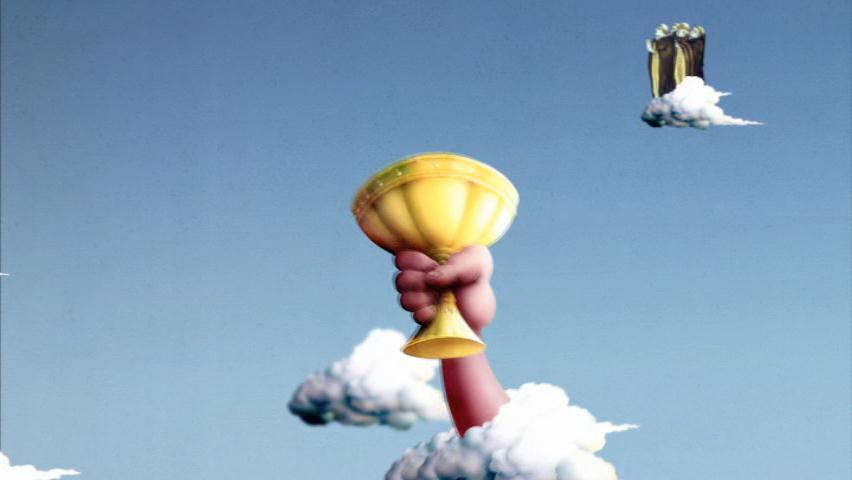
\includegraphics[width=0.8\textwidth]{grail.jpg}
  % \caption[Voorbeeld figuur.]{\label{fig:grail}Voorbeeld van invoegen van een figuur. Zorg altijd voor een uitgebreid bijschrift dat de figuur volledig beschrijft zonder in de tekst te moeten gaan zoeken. Vergeet ook je bronvermelding niet!}
% \end{figure}

% \begin{listing}
  % \begin{minted}{python}
    % import pandas as pd
    % import seaborn as sns

    % penguins = sns.load_dataset('penguins')
    % sns.relplot(data=penguins, x="flipper_length_mm", y="bill_length_mm", hue="species")
  % \end{minted}
  % \caption[Voorbeeld codefragment]{Voorbeeld van het invoegen van een codefragment.}
% \end{listing}

% \begin{table}
 %  \centering
  % \begin{tabular}{lcr}
   %  \toprule
    % \textbf{Kolom 1} & \textbf{Kolom 2} & \textbf{Kolom 3} \\
    % $\alpha$         & $\beta$          & $\gamma$         \\
    % \midrule
    % A                & 10.230           & a                \\
    % B                & 45.678           & b                \\
    % C                & 99.987           & c                \\
    % \bottomrule
  % \end{tabular}
 % \caption[Voorbeeld tabel]{\label{tab:example}Voorbeeld van een tabel.}
% \end{table}

% ================================================================

Inleidende alinea

% ================================================================

\section{Automatische beoordelingen binnen het programmeeronderwijs}
\label{ch:autograding}

\subsection{Evolutie van autograding}

\subsection{Beperkingen van autograding}

% ==> uitleggen waarom autograding niet voldoende is

% ================================================================

\section{De opkomst van LLM's in het onderwijs}
\label{ch:llm-opkomst}

\subsection{Wat zijn LLM's?}

\subsection{De mogelijkheden van LLM's binnen het programmeeronderwijs}

\subsection{Risico's en beperkingen van LLM's}

% ==> uitleggen dat LLM's krachtiger zijn dan autograding, maar dat er ook limitaties zijn

% ================================================================

\section{LLM's voor automatische code-evaluatie en beoordeling}
\label{ch:llm-scoring-beoordeling}

\subsection{De vergelijking tussen LLM's en menselijke beoordeling}

\subsection{Open-source versus closed-source modellen}

\subsection{Fine-tuning en verbetering van de feedbackkwaliteit}

\subsection{MastraAI}

% ==> opbouwen naar / onderbouwen van vergelijkende studie

% =================================================================

\section{Impact van LLM-gegenereerde feedback op studenten}
\label{ch:impact-op-studenten}

\subsection{Effect op prestaties en problem-solving}

\subsection{Studentenpercepties en gedrag}

% ==> belang van feedback kwaliteit aantonen

% =================================================================

\section{Betrouwbaarheid}
\label{ch:betrouwbaarheid-detectie-output}

\subsection{Hallucinaties}

% ==> ook belangrijk, misschien hier nog een extra alinea?
% TODO: misschien hier extra alinea?

% =================================================================

\section{Pedagogische en ethische implicaties}
\label{ch:pedagogische-ethische-implicaties}

\subsection{Pedagogische randvoorwaarden}

\subsection{Europese AI Act en high-risk classificatie}

% ==> heel belangrijk om ook te vermelden

% =================================================================

\section{Onderzoeksrelevantie en positionering}
\label{ch:onderzoeksrelevantie-positionering}

\subsection{Wat weten we al?}

\subsection{Wat weten we nog niet?}

\subsection{Positionering van deze bachelorproef}

% ==> goeie afsluiter

% =================================================================




%%=============================================================================
%% Methodologie
%%=============================================================================
\chapter{\IfLanguageName{dutch}{Methodologie}{Methodology}}%
\label{ch:methodologie}

Deze bachelorproef werd uitgewerkt in vijf opeenvolgende fases. Elke fase had een duidelijke doelstelling met eigen deliverables en een specifieke techniek. Zo werd de focus telkens op een ander deel van het probleem gelegd en werd er systematisch verder gebouwd aan een conclusie. In totaal werden er 14 werkdagen voorzien, waarvan 1 werkdag per werkweek besteed werd aan het onderzoek. Een overzicht van de tijdsbesteding per fase wordt weergegeven in Figuur~\ref{fig:gantt}.

\section{Fase 1: Analyse van het probleemdomein}

In de eerste fase van dit onderzoek werd het probleemdomein verder onderzocht, door middel van het huidige evaluatieproces binnen de opleidingsonderdelen Front-End Web Development en Web Services te analyseren. Hiervoor werden er interviews afgenomen met alle leden van de doelgroep, zijnde de 3 lectoren die beide vakken geven.

\vspace{1em}

Het doel van deze fase was:
\begin{itemize}
    \item verder verdiepen binnen het probleem, de evaluatiecriteria en de methoden die de lectoren momenteel hanteren.
    \item een gemiddelde tijdsbesteding per project in kaart brengen
    \item ervaringen met inconsistenties binnen beoordelingen te weten komen
\end{itemize}

Het resultaat van deze fase bestond uit een zeer duidelijke nood aan onderzoek, een concreet inzicht in de richting die het onderzoek uit zou moeten gaan, een overzicht van de verschillende evaluatiecriteria en hoe de evaluatie van studentenprojecten verloopt, en een verzameling van projecten met uiteenlopende beoordelingen, om te kunnen gebruiken als testprojecten voor bij een volgende fase.

\section{Fase 2: Literatuurstudie}

De tweede fase bestond uit een systematische literatuurstudie rond:
\begin{itemize}
    \item autograding binnen programmeeronderwijs
    \item het gebruik van Large Language Models (LLM's) voor code-analyse
    \item betrouwbaarheid, hallucinaties en bias in LLM-output
    \item prompt-engineering technieken
\end{itemize}

Uit deze literatuurstudie werden verschillende relevante inzichten rondom het inzetten van LLM's verworven die voor de technische uitwerking van pas komen. Op basis van de technische vereisten werd gekozen voor de inzet van \textbf{qwen3-coder:480B Cloud}. Dit model werd geselecteerd vanwege zijn sterke redeneercapaciteiten, het feit dat het als cloud-model geen lokale rekenkracht vereist, en de gratis beschikbaarheid voor dit onderzoek.

\section{Fase 3: Ontwerp en opzetten testomgeving en PoC}

In de derde fase werd een reproduceerbare testomgeving ontwikkeld waarin het geselecteerde LLM systematisch ingezet kon worden voor de analyse van studentenprojecten. Dit omvat:
\begin{itemize}
    \item het implementeren van een opsplitsingsmechanisme om rekening te houden met contextlimieten
    \item het ontwikkelen van scripts voor automatische projectanalyse
    \item het ontwerpen van een gestandaardiseerde promptstructuur
    \item het definiëren van output standaarden
\end{itemize}

De PoC werd stapgewijs opgebouwd, uitgebreid en verbeterd, waardoor deze fase een grondig gedocumenteerde en reproduceerbare testomgeving oplevert als deliverable.

\section{Fase 4: Kwantitatieve evaluatie van de PoC}

In deze fase werd de werking van de PoC geëvalueerd op basis van:

\begin{itemize}
    \item correctheid van criteriadetectie door het LLM
    \item consistentie van de AI-beoordelingen met de evaluaties van lectoren
    \item de kwaliteit van de gegenereerde feedback
\end{itemize}

De resultaten van de automatische analyse werden getoetst aan de hand van de eerder verzamelde handmatige beoordelingen om de betrouwbaarheid van de tool vast te stellen.

% =================================================================

\section{Fase 5: Conclusie}

In de laatste fase werden de bevindingen uit alle voorgaande fasen samengebracht. 

Hier werd beoordeeld:
\begin{itemize}
    \item in welke mate LLM’s bruikbaar zijn als ondersteuning bij evaluatie van studentenprojecten
    \item op welke criteria LLM’s sterker of zwakker presteren
    \item welke randvoorwaarden noodzakelijk zijn voor verantwoord gebruik binnen het kader van de AI Act
\end{itemize}


%%=============================================================================
%% Probleemdomein
%%=============================================================================
\chapter{Probleemdomein}%
\label{ch:probleemdomein}

Om een duidelijk inzicht te krijgen in het huidige evaluatieproces van studentenprojecten binnen de opleidingsonderdelen Front-End Web Development en Web Services, werden interviews afgenomen met de drie lectoren die deze projecten evalueren. Het doel van deze interviews was om de huidige werkwijze, de tijdsbesteding, de gebruikte evaluatiecriteria en de ervaren moeilijkheden tijdens het beoordelen van projecten in kaart te brengen.

\section{Tijdsbesteding bij het evalueren van projecten}

Uit de interviews blijkt dat het beoordelen van één studentenproject gemiddeld ongeveer één uur in beslag neemt. Deze tijd kan echter sterk variëren afhankelijk van de kwaliteit en/of complexiteit van het project. Voor grotere of complexere projecten kan de evaluatietijd oplopen tot anderhalf uur, terwijl eenvoudiger projecten sneller beoordeeld kunnen worden. Dit vooral doordat er extra onderzoek gedaan moet worden naar extra technologieën die gebruikt werden en omdat er bij grotere projecten vaak meerdere extra technologieën aanwezig zijn. Projecten die niet correct opstarten of onvoldoende gedocumenteerd zijn vereisen vaak meer tijd omdat de lector eerst moet achterhalen hoe het project werkt.

\vspace{1em}

De evaluatie begint meestal met het binnenhalen van het project, het installeren van dependencies en het opstarten van de applicatie aan de hand van de instructies die de student heeft voorzien in de README. Indien dit proces niet vlot verloopt, kan dit de totale evaluatietijd aanzienlijk verhogen. Daarnaast werd aangegeven dat zowel zeer goede als zeer zwakke projecten vaak meer tijd vragen dan gemiddelde projecten. Bij sterke projecten wordt meer tijd besteed aan het begrijpen van de gebruikte technieken, terwijl bij zwakke projecten extra aandacht besteed wordt aan het formuleren van correcte en duidelijke feedback. Dit wordt gedaan om de studenten die naar tweede zit worden doorverwezen extra duidelijkheid te geven en te helpen om hun project voldoende te kunnen verbeteren voor de volgende evaluatie.

\vspace{1em}

De meerderheid van de lectoren geven aan dat de evaluaties vaak in lange sessies gebeuren, waarbij meerdere projecten na elkaar beoordeeld worden. Hierdoor kan de snelheid van evalueren variëren doorheen de dag. In het begin van een evaluatieperiode wordt vaak trager gewerkt omdat er nog geen duidelijke referentie bestaat voor het niveau van de projecten. Naarmate meer projecten beoordeeld worden, ontstaat een soort referentiekader, waardoor latere evaluaties sneller verlopen. Soms wordt ook teruggekeerd naar eerder beoordeelde projecten om de beoordeling beter te kunnen vergelijken en de consistentie te bewaren. In bijzondere gevallen worden bij twijfel de collega's ingeschakeld, om de evaluatie correct en consistent te houden.

\section{Verdeling tussen controle van criteria en inhoudelijke feedback}

Tijdens de interviews werd ook gevraagd naar welk deel van de evaluatietijd besteed wordt aan het controleren van evaluatiecriteria, en welk deel aan het formuleren van inhoudelijke feedback. De lectoren geven aan dat het controleren van basiscriteria relatief snel kan verlopen, maar dat het opzoeken van de implementatie in de code toch een aanzienlijke hoeveelheid tijd vraagt. Ook niet iedereen gaat op dezelfde manier te werk. Een deel van de lectoren overloopt de lijst op voorhand, een ander deel bekijkt de lijst tijdens het evalueren. Vooral bij grotere projecten kan het zoeken naar specifieke onderdelen in de codebase zeer tijdrovend zijn.

\vspace{1em}

Het grootste deel van de evaluatietijd wordt besteed aan het formuleren van inhoudelijke feedback. Lectoren proberen niet alleen na te gaan of een criterium aanwezig is, maar ook hoe goed het geïmplementeerd is en of de student de onderliggende concepten begrijpt. Het uitschrijven van duidelijke en bruikbare feedback wordt als een van de meest tijdsintensieve onderdelen van de evaluatie beschouwd. In sommige gevallen wordt meer dan de helft van de totale evaluatietijd besteed aan het opstellen van deze feedback. Dit omdat er bij projecten die gelijkaardig zijn aan het voorbeeldproject vaak verteld wordt wat er beter was dan het voorbeeld, en wat er slechter was. Bij slechtere projecten wordt er altijd extra aandacht besteed aan duidelijke feedback, om de student zo goed mogelijk op weg te helpen om hun project tegen de volgende evaluatie goed verbeterd te hebben.

\section{Consistentie en subjectiviteit in beoordelingen}

Een belangrijk probleem dat in alle interviews naar voren kwam, is de moeilijkheid om consistent te blijven bij het beoordelen van een groot aantal projecten. De lectoren geven aan dat hun beoordeling beïnvloed kan worden door eerdere projecten die ze bekeken hebben. Na meerdere zwakke projecten kan een gemiddeld project bijvoorbeeld beter lijken dan het in werkelijkheid is, terwijl na een sterk project een gelijkaardig werk strenger beoordeeld kan worden.

\vspace{1em}

Ook de mentale vermoeidheid tijdens lange evaluatiesessies speelt een rol. Sommige lectoren geven aan dat ze minder projecten per dag proberen te beoordelen om de kwaliteit van hun feedback te behouden. Daarnaast wordt aangegeven dat de eigen emotionele toestand of frustratie over slecht uitgewerkte projecten onbewust invloed kan hebben op de beoordeling.

\section{Huidige hulpmiddelen en automatisering}

Momenteel gebeurt de evaluatie van projecten grotendeels manueel. Er bestaan wel hulpmiddelen om projecten automatisch binnen te halen of te controleren of ze kunnen opstarten, maar er wordt geen gebruik gemaakt van een volwaardig autograding- of feedbacksysteem. Enkele lectoren hebben wel geëxperimenteerd met Large Language Models om bepaalde onderdelen van de evaluatie te automatiseren, zoals het controleren van ontvankelijkheidscriteria of het vergelijken van een project met een voorbeeldoplossing.

\vspace{1em}

Deze experimenten toonden aan dat LLM’s zeker potentieel hebben om bepaalde repetitieve controles sneller uit te voeren, maar dat de betrouwbaarheid van de resultaten nog niet voldoende is om ze zonder controle te gebruiken. Er werd bijvoorbeeld vastgesteld dat een model soms vergelijkbare scores geeft aan zowel goede als zwakke projecten, wat wijst op een gebrek aan diepgang in de evaluatie. Daarnaast kan de verwerkingstijd van grote projecten een probleem vormen, vooral wanneer de volledige codebase in één keer geanalyseerd moet worden. Hier komen dan ook context- en tokenlimitaties naar boven. Hierdoor moet de code opgesplitst worden in kleinere delen, wat de complexiteit van een mogelijke automatisering verhoogt.

\section{Belang van inzicht in het werk van de student}

Een ander aspect dat volgens alle geïnterviewde lectoren moeilijk te automatiseren is, is het beoordelen van in welke mate een student de ingediende code zelf begrijpt en geschreven heeft. Om dit te controleren werd voorheen gebruik gemaakt van een mondelinge verdediging. Dit werd voor enkele jaren afgeschaft, maar met de opkomst van LLM's zal dit komend academiejaar terug worden ingelast. Naast het potentiëel van LLM's om projecten te evalueren, zouden ze ook hierbij kunnen helpen. Het afnemen van persoonlijke mondelinge examens vereist ook veel voorbereidend werk, zoals het opstellen van relevante vragen en het doornemen van het project van elke student. LLM's zouden hier ook tijdsbesparend kunnen werken, door een kleine samenvatting van elk project te kunnen opstellen en interessante onderdelen van bepaalde projecten te kunnen highlighten. Hier kan de lector dan dieper op in tijdens het mondelinge examen.

\section{Juridische en ethische overwegingen}

Naast de praktische en technische uitdagingen bij de implementatie van een LLM-gebaseerde evaluatieflow, spelen er ook belangrijke juridische en ethische overwegingen, in het bijzonder op het vlak van data governance, privacy en intellectueel eigendom. Om hierover duidelijkheid te scheppen, werd advies ingewonnen bij de functionaris gegevensbescherming (DPO) en het diensthoofd studentenaangelegenheden van HOGENT.

\vspace{1em}

Ten eerste zijn er de aspecten rond gegevensbescherming en de Algemene Verordening Gegevensbescherming (AVG/GDPR). Het gebruik van studentenprojecten als data voor een AI-systeem impliceert de verwerking van persoonsgegevens. Omdat het systeem gebruikt kan worden in de context van evaluaties en besluitvorming, bevindt deze toepassing zich mogelijk in de hoogrisicozone volgens de Europese AI Act. Dit vereist naleving van verschillende basisbeginselen, zoals rechtmatigheid, transparantie (gebruikers moeten geïnformeerd zijn over de interactie met het AI-systeem), doelbinding en dataminimalisatie. De AI Act legt bovendien een sterke nadruk op zinvol menselijk toezicht gedurende het hele proces. Voor het onderzoek en een eventuele toepassing betekent dit onder meer dat persoonsgegevens idealiter gepseudonimiseerd worden en dat een veilige infrastructuur voor gegevensverwerking noodzakelijk is.

\vspace{1em}

Ten tweede is er het aspect van intellectueel eigendom. Volgens artikel 55 van het Onderwijs- en Examenreglement (OER) van HOGENT blijft de code en het werk dat studenten creëren in het kader van hun opleiding hun intellectueel eigendom. Het gebruik van deze projecten buiten de initiële onderwijscontext waarvoor ze werden ingediend (in dit geval voor analyse door een AI-model in het kader van dit onderzoek) vereist dan ook de expliciete toestemming van de betrokken studenten. Aangezien dit onderzoek wordt uitgevoerd door een student-onderzoeker en niet namens de instelling, kan er geen beroep gedaan worden op eventuele gebruiksrechten van HOGENT.

\vspace{1em}

Tot slot, wat betreft de rol van de lectoren in een AI-ondersteunde evaluatieflow, bepaalt artikel 30 van het OER dat de uiteindelijke evaluatiebevoegdheid en \newline -verantwoordelijkheid onverkort bij de lector blijven berusten. Hoewel AI-output als hulpmiddel kan dienen ter ondersteuning en voor tijdsbesparing, doet dit geen afbreuk aan de persoonlijke verantwoordelijkheid van de evaluator. Er is dus telkens een noodzaak voor controle door de docent, wat ook in lijn is met de vereisten van de AI Act omtrent menselijke betrokkenheid bij geautomatiseerde besluitvorming.

\section{Conclusie van het probleemdomein}

Op basis van de interviews kan geconcludeerd worden dat het huidige evaluatieproces van studentenprojecten tijdsintensief, repetitief en deels subjectief is. Een groot deel van de tijd gaat naar het controleren van criteria en het formuleren van feedback, terwijl de consistentie tussen beoordelingen niet altijd gegarandeerd kan worden. Hoewel er interesse bestaat in het gebruik van automatisering en Large Language Models, worden deze momenteel nog niet structureel ingezet vanwege beperkingen op vlak van betrouwbaarheid, snelheid en contextverwerking.

\vspace{1em}

Daarnaast brengt een eventuele integratie van AI-systemen in het evaluatieproces cruciale juridische en ethische vereisten met zich mee. Het waarborgen van gegevensbescherming, het respecteren van het intellectueel eigendom van de studenten en het behouden van menselijk toezicht bij de beoordeling blijken absolute randvoorwaarden te zijn.

\vspace{1em}

Desondanks kan er worden geconcludeerd dat er duidelijk veel potentieel zit in het bieden van ondersteuning bij deze tijdrovende evaluaties. Naast tijdswinst is er ook mogelijks verhoogde consistentie bij het inzetten van LLM's en zouden LLM's bovendien extra hulp kunnen bieden bij de voorbereiding van mondelinge examens. Dit vormt de aanleiding voor het verdere onderzoek naar de bruikbaarheid en betrouwbaarheid van LLM-gebaseerde evaluatie binnen deze context, waarbij steeds de geldende privacy- en auteursrechten gerespecteerd moeten worden.

%%=============================================================================
%% POC
%%=============================================================================
\chapter{Proof-of-Concept}%
\label{ch:poc}

\section{De Evaluatieflow}

De geautomatiseerde evaluatie van studentenprojecten binnen de proof-of-concept wordt aangestuurd door een gecentraliseerd script (\texttt{run-evaluation.js}). Dit proces is opgebouwd uit verschillende opeenvolgende fasen om een veilige, contextbewuste en doeltreffende code-evaluatie te garanderen.

\vspace{1em}

\subsection{Stap 1: Initialisatie en Isolatie (Sandbox Setup)}

De veiligheid en integriteit van het evaluatieproces vormen een primaire zorg bij het geautomatiseerd uitvoeren en inspecteren van studentencode. Daarom start de flow met het opzetten van een geïsoleerde 'sandbox' omgeving via E2B. Deze sandbox fungeert als een afgeschermde virtuele machine met een vaste time-out limiet.

\vspace{1em}

Zodra de sandbox operationeel is, wordt de broncode van de student ingeladen in de tijdelijke omgeving. Ook wordt tijdens deze stap het voorbeeldproject voor beide OLOD's ingeladen. Dit stelt de latere AI-agents in staat om de implementatie van de student te vergelijken met een beoogd resultaat.

\subsection{Stap 2: Verkennende Analyse (Dossier Intake)}

Alvorens de aanwezigheid van individuele criteria te controleren, is het cruciaal dat het systeem de bredere context van het project begrijpt. Hiervoor is een specifieke AI-agent ontwikkeld: de \texttt{dossierAgent}. Deze agent voert een initiële verkenning uit in de sandbox om een globaal ``projectdossier'' op te bouwen.

\vspace{1em}

Tijdens deze fase maakt de agent iteratief gebruik van tools om de mappenstructuur te verkennen, documentatie (zoals README-bestanden) in te lezen en configuratiebestanden (zoals \texttt{package.json} of Dockerfiles) te analyseren. Het resultaat wordt geparst tot een gestructureerd JSON-object dat onder meer de technologiestack, startinstructies, potentiële risico's, en de belangrijkste componenten (frontend, backend, database, tests) beschrijft. Dit voorkomt dat het systeem bij het beoordelen van elk afzonderlijk criterium de projectstructuur opnieuw moet ontdekken en vermindert onnodige tool calls.

\subsection{Stap 3: Dynamische Routing (Coordinator Agent)}

De eigenlijke evaluatie is opgedeeld in specifieke criteria-taken. Voor elk criterium wordt het beschrijvende markdown-bestand ingelezen. In plaats van alle criteria door één generiek model te laten beoordelen, maakt het systeem gebruik van een routing-mechanisme.

\vspace{1em}

Een gespecialiseerde \texttt{coordinatorAgent} analyseert de inhoud van het criterium en beslist (via een routeringsfunctie) welke andere agent het meest geschikt is om dit specifieke onderdeel te beoordelen. Zo kan een criterium over REST API-architectuur worden toegewezen aan een backend-agent, terwijl een UI-gerelateerd criterium naar een frontend-agent gaat. De coördinator voegt hierbij ook zijn redenering aan toe, wat handig is om de keuze voor bepaalde beslissingen beter te kunnen begrijpen.

\subsection{Stap 4: Specialistische Evaluatie met Tooling}

Na de toewijzing genereert het systeem een uitgebreide prompt voor de geselecteerde specialist-agent. Deze instructie bundelt alle verzamelde informatie:
\begin{itemize}
    \item De identificatiegegevens van de sandbox en projectpaden.
    \item De algemene projectcontext die verzameld werd tijdens de dossier intake.
    \item De specifieke criterium-tekst.
    \item De rol, focus en de routeringsreden van de gekozen agent.
\end{itemize}

De specialist-agent begint vervolgens aan een iteratief evaluatieproces. Binnen een vastgelegde limiet (bijvoorbeeld 15 stappen) roept de agent autonoom tools aan. Hij kan bestanden openen, broncode regel voor regel inspecteren, of eventueel commando's uitvoeren binnen de sandbox om bewijsmateriaal te verzamelen voor het specifieke criterium.

\subsection{Stap 5: Gestructureerde Parsing en Besluitvorming}

Zodra de specialist-agent zijn onderzoek heeft afgerond, retourneert hij zijn bevindingen. Om deze ruwe output om te zetten in applicatiedata, wordt een strikt parsing-mechanisme toegepast waarbij het antwoord moet voldoen aan een vooraf gedefinieerde JSON-structuur.

\vspace{1em}

Hierbij dwingt het systeem de agent om de evaluatiestatus te normaliseren naar één van de drie mogelijke uitkomsten:
\begin{itemize}
    \item \textbf{Aanwezig}: Er is direct en overtuigend bewijs gevonden in de code of configuratie.
    \item \textbf{Afwezig}: De agent heeft de relevante plaatsen in het project adequaat onderzocht, maar het criterium werd niet aangetroffen.
    \item \textbf{Onduidelijk}: De bevindingen zijn tegenstrijdig of het bewijs in de code is onvoldoende om een definitieve 'ja/nee' conclusie te trekken.
\end{itemize}

Naast de status bevat het resulterende JSON-object ook een gedetailleerde argumentatie (met verwijzingen naar specifieke codebestanden of logica) en constructieve feedback.

\subsection{Stap 6: Aggregatie en Afronding}

In de laatste fase loopt het script alle criteria af en registreert eventuele validatie- of runtime-fouten per criterium. Uiteindelijk worden alle individuele evaluaties, eventuele foutmeldingen, en de dossier-intake geaggregeerd in één overkoepelend JSON-rapport.

\vspace{1em}

Dit bestand krijgt uitgebreide metadata (zoals timestamps, gebruikte modellen, time-outlimieten) en wordt opgeslagen voor verdere verwerking of visuele weergave. Ten slotte sluit de flow veilig af door het kill-commando naar E2B te sturen, waardoor de tijdelijke sandbox definitief wordt vernietigd en er geen onnodige cloudbronnen open blijven staan.

\section{Technologische Keuzes}

Bij de ontwikkeling van de proof-of-concept is bewust gekozen voor een reeks moderne frameworks en technologieën die het geautomatiseerd evalueren van broncode op een schaalbare en veilige manier mogelijk maken.

\subsection{Mastra: Typed Agent Framework}
Voor de orchestratie van de AI-agents is gekozen voor \textbf{Mastra}, een TypeScript-first agent framework. In tegenstelling tot meer generieke alternatieven zoals LangChain of CrewAI, die vaak sterk op Python en abstracte concepten gericht zijn, biedt Mastra een lichtgewicht en sterk getypeerde omgeving. Dit is essentieel voor het bouwen van betrouwbare integraties met gestructureerde output (JSON) en specifieke tools. Mastra stelt ons in staat om de \textit{routing} en executie van \textit{tools} door de verschillende agents expliciet en veilig te beheren binnen een Node.js ecosysteem.

\vspace{1em}

\subsection{E2B Sandbox: Veilige Code-executie}
Het draaien van ongecontroleerde studentencode houdt inherente veiligheidsrisico's in. Daarom wordt er gebruikgemaakt van de \textbf{E2B Sandbox}. Waar een traditionele aanpak vaak vereist dat er lokaal Docker-containers of virtuele machines moeten worden opgesponnen (wat foutgevoelig is en een trage opstarttijd heeft), is E2B speciaal ontworpen voor AI-code executie. Het biedt onmiddellijk opstartende, volledig afgeschermde cloudomgevingen met configureerbare time-outs. Hierdoor kan de agent veilig bestanden inlezen en processen starten zonder dat de hostmachine of het netwerk gevaar loopt.

\vspace{1em}

\subsection{LLM: Qwen en Reasoning}
Voor het genereren van de beoordelingen en het analyseren van de code is gekozen voor het \textbf{qwen3-coder:480b-cloud} model (specifiek gefocust op code). Qwen3-coder:480b-cloud onderscheidt zich door zijn sterke \textit{thinking} (reasoning) capaciteiten op het gebied van softwareontwikkeling. In plaats van direct een oppervlakkig antwoord te genereren, dwingt de architectuur van dit LLM een analytisch proces af waarbij eerst de code-logica grondig wordt overwogen alvorens het effectieve JSON-oordeel terug te geven. Doordat qwen3-coder:480b-cloud een cloud model is, zijn er ook geen hoge systeemvereisten.

\vspace{1em}

\section{Voorbeeld van een Evaluatie (Input \& Output)}

Om de abstracte flow concreet te maken, tonen we hieronder een voorbeeld van hoe een criterium-input eruitziet, en hoe de uiteindelijke JSON-output van de AI-agent wordt opgeslagen.

\vspace{1em}

\subsection{Het Criterium (Markdown)}
De evaluatiecriteria worden opgesteld in natuurlijke taal als markdown-bestanden. Dit maakt het voor docenten eenvoudig om criteria toe te voegen of te wijzigen zonder de code van de evaluator aan te passen. Een volledig voorbeeld van een ontvankelijkheidscriterium voor de frontend is te zien in Codefragment~\ref{lst:criterium-markdown}.

\begin{listing}[htbp]
\begin{minted}{markdown}
Ontvankelijkheidscriterium (Front-end): De applicatie wijkt voldoende af van de voorbeeldapplicatie.

Controle-instructies:

- Open het voorbeeldproject in de referentielocatie die in de flow wordt meegegeven.
- Vergelijk de frontend-structuur, componenten, pagina's en functionaliteit met het voorbeeld.
- Baseer je beoordeling op concrete code- en bestandsverschillen, niet op veronderstellingen.

Beslisstatus:

- aanwezig: de frontend verschilt duidelijk genoeg van het voorbeeldproject in structuur en functionaliteit.
- afwezig: de frontend lijkt grotendeels een kopie of is onvoldoende onderscheidend.
- onduidelijk: het verschil kan niet betrouwbaar worden vastgesteld.

Geef een kort, concreet bewijs met bestandsverwijzingen.
\end{minted}
\caption{Voorbeeld van een ontvankelijkheidscriterium in markdown-formaat.}
\label{lst:criterium-markdown}
\end{listing}

\subsection{De Resultaten (JSON)}
De AI-agent voert op basis hiervan zijn verkenning uit in de sandbox en genereert een gestructureerde JSON-respons. Codefragment~\ref{lst:criterium-json} toont de werkelijke output van de agent na evaluatie, inclusief de uitgebreide beoordeling, de onderbouwing (bewijs), feedback voor de student en interne metadata over de gebruikte agent en routering.

\begin{listing}[htbp]
\begin{minted}{json}
{
  "criteria": "Ontvankelijkheidscriterium (Front-end)",
  "aanwezig": "aanwezig",
  "bewijs": "Het studentenproject gebruikt een unieke manga-thematisering met specifieke componenten zoals MangaList.jsx, StudioList.jsx en NavBar.jsx die niet voorkomen in het voorbeeldproject. De structuur van de pages directory (/mangas, /studios, /characters) wijkt af van het voorbeeldproject (/places, /transactions). Bovendien gebruikt het studentenproject Bootstrap terwijl het voorbeeld TailwindCSS gebruikt, wat aanzienlijke verschillen oplevert in styling en benadering.",
  "feedback": "De frontend wijkt voldoende af van het voorbeeldproject door het gebruik van een andere thematiek (manga ipv places/budget), andere componentenstructuur en andere CSS-framework (Bootstrap ipv Tailwind). Dit voldoet aan het ontvankelijkheidscriterium.",
  "_meta": {
    "model": "qwen3-coder:480b-cloud",
    "sandboxId": "imeky4tycewxe2crzz5wk",
    "project": "fews-project-05",
    "domain": "frontend",
    "criteriaFile": "ov-fe-wijkt-voldoende-af-van-voorbeeldapplicatie.md",
    "referenceProjectPath": "/home/user/__voorbeeldapplicatie",
    "specialistAgent": "apiAgent",
    "coordinatorReason": "frontend fallback naar interface/API specialist"
  }
}
\end{minted}
\caption{Gegenereerde JSON-output van de specialist-agent voor het criteria-markdown bestand.}
\label{lst:criterium-json}
\end{listing}

\section{Uitdagingen en Beperkingen}

Hoewel de geautomatiseerde flow uiterst succesvolle resultaten boekt, kwamen er tijdens de ontwikkeling van de proof-of-concept enkele belangrijke uitdagingen en limitaties naar voren.

\subsection{Time-out Limieten van de Sandbox}
De E2B Sandbox is een zeer efficiënte oplossing, maar introduceert restricties op het vlak van uitvoeringstijd en systeembronnen. Bepaalde studentenprojecten met omvangrijke afhankelijkheden kunnen erg lang duren om initieel op te starten (denk aan een zware \texttt{npm install} of het uitvoeren van complexe database migraties). Dit zorgde in de beginfase soms voor voortijdige time-outs in de E2B omgeving, waardoor het evaluatieproces onverwacht werd afgebroken.

\subsection{Tragere Runs door Reasoning (Thinking)}
Een andere aanzienlijke uitdaging is de algehele duur van een evaluatieronde. Omdat het gebruikte LLM (qwen3-coder:480b-cloud) gebruikmaakt van een uitgebreid \textit{thinking}- of redeneerproces, ligt de kwaliteit en de betrouwbaarheid van de uiteindelijke beoordeling erg hoog. Echter vergt dit diepgaande redeneerproces (het model "denkt na" in verborgen tokens voordat de uiteindelijke JSON wordt gegenereerd) aanzienlijk veel tijd. In combinatie met de tijd die nodig is voor het iteratief aanroepen van verschillende \textit{tools} in de cloud-sandbox, kan de complete evaluatie van één project gemakkelijk tientallen minuten in beslag nemen.

%%=============================================================================
%% Resultaten en Data-analyse
%%=============================================================================
\chapter{Resultaten en Data-analyse}%
\label{ch:evaluatie}

Dit hoofdstuk beantwoordt de centrale onderzoeksvraag door de resultaten van de geautomatiseerde AI-evaluatie systematisch te vergelijken met de handmatige beoordelingen van de lectoren. De proof-of-concept werd uitgevoerd op een selectie van acht studentenprojecten uit het opleidingsonderdeel Front-End Web Development \& Web Services (FEWS). Voor elk project werden zowel de ontvankelijkheidscriteria als de evaluatiecriteria door het AI-systeem beoordeeld. De lectoren beoordeelden dezelfde projecten aan de hand van evaluatiekaarten in Excel. Door beide naast elkaar te leggen, kan de betrouwbaarheid en nauwkeurigheid van de evaluatie worden vastgesteld.

\section{Overzicht van de Dataset}
\label{sec:dataset}

De analyse omvat acht FEWS-projecten waarvoor volledige AI-resultaten en ingevulde evaluatiekaarten van de lectoren beschikbaar zijn. Per project werden twee afzonderlijke runs uitgevoerd:

\begin{itemize}
    \item \textbf{Ontvankelijkheidscriteria} (11 criteria): controle of een project aan de minimumvereisten voldoet. Vijf criteria betreffen de frontend, zes de web services.
    \item \textbf{Evaluatiecriteria} (19 criteria): inhoudelijke beoordeling van de implementatiekwaliteit. Acht criteria evalueren de frontend, elf de backend.
\end{itemize}

De evaluatiekaarten van de lectoren bevatten drie tabbladen: een ontvankelijkheidstabel met voldaan of niet voldaan en twee scoretabellen (Web Services en Front-end) met een ABCD-schaal en gewogen puntentoekenning. De gedetailleerde resultaten per project zijn opgenomen in het overzicht op p.~\pageref{tab:dataset-overzicht}. Tabel~\ref{tab:dataset-overzicht} vat de omvang van de geanalyseerde dataset samen.

\section{Ontvankelijkheidsvergelijking}
\label{sec:ontv-vergelijking}

De ontvankelijkheidstest vormt het meest directe vergelijkingspunt: zowel de AI als de lector beantwoorden dezelfde binaire vraag: ``Voldoet het project aan dit criterium of niet?'' De AI-status ``aanwezig'' werd gelijkgesteld aan de lector-status \textit{True}, en ``afwezig'' aan \textit{False}.

\subsection{Globale Nauwkeurigheid}

Over de acht projecten werden 87 ontvankelijkheidscriteria beoordeeld door de AI. Bij 79 hiervan kon een koppeling worden gemaakt met het overeenkomstige lector-oordeel. De resultaten staan samengevat in Tabel~\ref{tab:ontv-globaal}.

\vspace{1em}

Met een nauwkeurigheid van \textbf{91,1\%} komt het AI-oordeel in meer dan negen op de tien gevallen overeen met dat van de menselijke beoordelaar. Dit beantwoordt deelvraag~1 van het oplossingsdomein: het LLM is in staat om vooraf gedefinieerde ontvankelijkheidscriteria met een hoge mate van correctheid te detecteren.

\vspace{1em}

Zie Tabel~\ref{tab:ontv-per-project} voor een gedetailleerde uitsplitsing per project. Vier projecten behalen een perfecte score (100\%), drie scoren 90\%, en één project (fews-project-06) wijkt af met 60\%.

\vspace{1em}

De uitschieter bij fews-project-06 (60\%) verdient nadere verklaring en legt een interessant fenomeen bloot. Bij dit project bestond de inlevering uitsluitend uit een backend (Web Services). Er was dus geen frontend aanwezig in de repository. De AI merkte dit correct op en markeerde de vier frontend-criteria (\textit{extra technologie}, \textit{React-gebruik}, \textit{voldoende complexiteit} en \textit{afwijking van de voorbeeldapplicatie}) terecht als ``afwezig''. Op de evaluatiekaart waren de frontend-ontvankelijkheidscriteria echter toch als voldaan aangevinkt, vermoedelijk als een procedurele handeling (workaround) door de lector omdat de student dit deel niet hoefde in te dienen en anders de evaluatietool mogelijk blokkeert. Dit verklaart de ogenschijnlijk lage nauwkeurigheidsscore van dit project maar bevestigt wel de betrouwbaarheid van de AI als objectieve code-validator.

\vspace{1em}

Bij project 04 is de mismatch te wijten aan het criterium \textit{integratietesten}. De AI rapporteerde dit als aanwezig omdat het één testbestand vond, terwijl de lector dit als niet-voldaan beoordeelde met de opmerking ``maar 1 test''. Dit toont aan dat de AI soms te binair oordeelt waar de lector een kwalitatieve ondergrens hanteert.

\subsection{Analyse per Criterium}

De analyse toont aan dat \textit{objectief verifieerbare} criteria hoger scoren dan \textit{subjectieve} criteria. Web services-criteria die steunen op bestandsanalyse (zoals NestJS-gebruik of de domeinafwijking) behalen een perfecte 100\%. De overige criteria scoren rond de 88\% omdat ze een hogere mate van interpretatie vereisen of gevoelig zijn voor de specifieke implementatiediepte (zoals het aantal testen).

\vspace{1em}

Dit beantwoordt deelvraag 4 van het oplossingsdomein: het LLM scoort sterk op objectief verifieerbare, structurele criteria en iets zwakker op criteria die subjectieve interpretatie vereisen.

\section{Vergelijking Evaluatiecriteria}
\label{sec:eval-vergelijking}

De evaluatiecriteria zijn complexer om te vergelijken dan de ontvankelijkheidscriteria. De AI kent een drieledig oordeel toe (aanwezig/afwezig/onduidelijk), terwijl de lectoren een ABCD-schaal hanteren.

\subsection{Het Schaalverschil}

De lectoren scoren op de volgende schaal:
\begin{itemize}
    \item[\textbf{A}] De standaard is overtroffen (hoger dan het voorbeeldproject).
    \item[\textbf{B}] De standaard is volledig behaald (gelijk aan het voorbeeldproject).
    \item[\textbf{C}] De standaard is gedeeltelijk behaald, maar voldoende.
    \item[\textbf{D}] De standaard is niet behaald (onvoldoende).
\end{itemize}

\noindent De AI kent géén gradatie toe: het beoordeelt uitsluitend de \textit{aanwezigheid} van een criterium. Een lector-score A, B of C impliceert dat het criterium aanwezig is, terwijl D impliceert een onvoldoende implementatie. De AI-status ``aanwezig'' stemt dus overeen met A/B/C, en ``afwezig'' met D. Zie het overzicht op p.~\pageref{tab:eval-overview} voor de resultaten per project.

\vspace{1em}

Dit fundamentele schaalverschil betekent dat de AI in zijn huidige vorm een \textit{screening-tool} is, geen \textit{scoring-tool}: het kan bepalen \textbf{of} iets er is, maar niet \textbf{hoe goed} het is.

De criteria die de AI als ``afwezig'' beoordeelde, bieden het meeste inzicht in de betrouwbaarheid. De gedetailleerde analyse hiervan is terug te vinden in het overzicht in de inleidende sectie (p.~\pageref{tab:afwezig-analyse}).

Twee terugkerende ``afwezig''-oordelen verdienen speciale aandacht:

\paragraph{Anti-patterns in React Hooks.} Dit criterium werd bij vrijwel alle projecten als ``afwezig'' beoordeeld. Dit is een \textit{semantisch interpretatieverschil}: het criterium zoekt naar de aanwezigheid van anti-patterns. Wanneer de AI rapporteert dat er geen anti-patterns zijn gevonden, is dat inhoudelijk \textit{positief}. Dit illustreert het belang van zorgvuldige criteriumformulering.

\paragraph{Isolatie datalaag.} Bij projecten 02, 03 en 04 oordeelde de AI dat de servicelaag SQL-queries of ORM-code bevatte. Bij inspectie van de lector-evaluatiekaarten blijken deze projecten inderdaad lagere scores (B of C) te hebben ontvangen op databank-gerelateerde criteria. Hier detecteert de AI dus correct tekortkomingen.

\vspace{1em}

Bij fews-project-01 gaven vijf evaluatiecriteria geen uitsluitsel. Dit was het gevolg van restricties in de sandbox-omgeving waardoor bepaalde bestanden niet diepgaand gelezen konden worden. Het systeem kiest er in dergelijke gevallen bewust voor om geen oordeel te vellen wanneer het onvoldoende bewijs kan verzamelen, wat de integriteit van de overige resultaten waarborgt.

\section{Kwalitatieve Analyse van de Feedback}
\label{sec:kwalitatief}

Naast de kwantitatieve vergelijking is de \textit{kwaliteit} van de gegenereerde feedback relevant voor deelvraag~2.

\subsection{Sterke Punten}

De AI-feedback vertoont drie sterke eigenschappen:
\begin{enumerate}
    \item \textbf{Traceerbaarheid}: de AI verwijst consequent naar exacte bestandspaden en lijnnummers, wat het oordeel direct verifieerbaar maakt.
    \item \textbf{Constructieve suggesties}: de feedback bevat concrete verbetervoorstellen die direct toepasbaar zijn.
    \item \textbf{Contextbewustzijn}: de AI begrijpt de samenhang tussen frontend en backend door de initiële dossier-intake.
\end{enumerate}

\subsection{Beperkingen \& Hallucinaties}

Hoewel in de literatuurstudie (Hoofdstuk \ref{ch:stand-van-zaken}) het risico op \textit{hallucinaties} en foutieve feedback uitgebreid aan bod kwam, bleek dit in de praktijk verrassend goed mee te vallen. De strakke structurering van de prompts via de agent-frameworks en de verplichte opmaak via JSON en rubrics, beperkten de speelruimte voor het LLM aanzienlijk. Verzonnen codefragmenten of feitelijk incorrecte verbetervoorstellen werden in de geteste steekproef niet waargenomen. Er diende wel rekening te worden gehouden met volgende algemene technische beperkingen:

\begin{enumerate}
    \item \textbf{Geen runtime-verificatie}: de AI kan (nog) niet controleren of de code daadwerkelijk succesvol uitvoerbaar is of op runtime fouten botst waardoor de beoordeling grotendeels statisch is.
    \item \textbf{Sandbox-restricties}: restricties in de E2B sandbox (of time-outs wegens de 'thinking' limiet) leiden er soms toe dat de AI geen uitsluitsel geeft en de status als 'onduidelijk' typeert.
\end{enumerate}




%%=============================================================================
%% Conclusie
%%=============================================================================

\chapter{Conclusie}%
\label{ch:conclusie}

Large Language Models (LLM's) worden tegenwoordig voor veel meer gebruikt dan alleen het schrijven van code. Ook voor het analyseren en evalueren van code bieden ze interessante mogelijkheden. Dit onderzoek had als doel om het evaluatieproces voor lectoren in het programmeeronderwijs te automatiseren en te verbeteren, zonder dat dit ten koste gaat van de kwaliteit van de feedback. Daarbij stond de volgende onderzoeksvraag centraal: in welke mate kunnen LLM's betrouwbare en bruikbare feedback genereren op de code van studentenprojecten binnen webontwikkeling, en hoe verhoudt zich dat tot de oordelen van de lectoren zelf?

\section{Beantwoording van de Onderzoeksvragen}

Uit de analyse van de \textit{proof-of-concept} (PoC) op echte HOGENT-studentenprojecten blijkt dat het AI-systeem erg goed presteert bij het detecteren van de ontvankelijkheidscriteria. Hierbij haalde het LLM namelijk een globale nauwkeurigheid van 91,1\% ten opzichte van het menselijke oordeel. 

\vspace{1em}

Het systeem is vooral sterk in het nakijken van objectieve, meetbare criteria, zoals het gebruik van een specifieke technologie of de aanwezigheid van formuliervalidatie. Omdat lectoren hier normaal veel tijd aan kwijt zijn, levert de AI een opvallende tijdswinst op. Bovendien haalt het systeem menselijke foutjes of inconsistenties uit de beoordelingen.
Wanneer we kijken naar meer kwalitatieve en complexe criteria (bijvoorbeeld 'hoe goed' is de architectuur), botst een simpele ``true/false'' -beoordeling soms op zijn limieten. Dit konden we oplossen door het toevoegen van een rubric-indicatie, waarbij de AI het project vergelijkt met een vooraf gemaakte voorbeeldapplicatie. Tot slot zorgde het ingebouwde redeneerproces (\textit{thinking}) van het gebruikte LLM voor erg gerichte en uiterst contextbewuste feedback, compleet met bestandsverwijzingen.

\section{Praktische Bruikbaarheid}

Uit de gesprekken en feedback van lectoren bleek de gestructureerde JSON-output van onschatbare waarde. Een bijkomende opluchting was dat de verwachte theorethische risico's op hallucinaties in praktijk stevig werden ingeperkt door het gestructureerde \textit{thinking}-concept van het Qwen3-Coder model. Wel kwamen er enkele belangrijke randvoorwaarden naar voren voordat zo'n systeem in de dagelijkse onderwijspraktijk geïmplementeerd kan worden:
\begin{itemize}
    \item \textbf{Verklaring van technische fouten}: Soms geeft de AI aan dat de beoordeling 'onduidelijk' is, op basis van een \textit{failure}. Dit wijst vrijwel altijd op technische problemen in de cloud-sandbox, zoals \textit{time-outs} bij te grote projecten, en betekent dus niet per se dat de studenten slechte code hebben geschreven.
    \item \textbf{Beperkte runtime-controle}: De app richt zich voornamelijk op de statische broncode. Als een applicatie door een bug bijvoorbeeld niet meer lokaal opstart, merkt de PoC dit niet direct op in het formele testrapport, tenzij de e2e-testen falen.
    \item \textbf{Inputvereisten voor studenten}: Om de automatische beoordeling vlot te laten verlopen, moeten studenten zich aan afspraken houden. Een duidelijke mapstructuur, een correct ingevuld mutatiedossier en up-to-date \texttt{package.json} bestanden zijn nodig voor de eerste stap, de 'dossier-intake'. 
\end{itemize}

\section{Toekomstig Werk}

Deze \textit{proof-of-concept} vormt een goede en werkende basis, maar er is uiteraard ruimte voor verdere uitbreiding. De volgende suggesties van lectoren vielen buiten de afgebakende scope van dit onderzoek, maar zijn ideale suggesties voor toekomstig werk. 

\vspace{1em}

Ten eerste kan de resulterende JSON-data direct ingeladen worden in een script dat automatisch de Excel-evaluatiekaarten invult met alle velden ('voldaan', 'feedback', 'rubric' en 'bewijs'). Technische fouten van de evaluatie tool zouden dan meteen geselecteerd  worden onderaan dat specifieke excel document.

\vspace{1em}

Daarnaast is het voor docenten cruciaal om bij teams (duo's) efficiënt de individuele inbreng te controleren. Door een koppeling met de API van GitHub in te bouwen toe, zou de tool in de toekomst kunnen verifiëren hoeveel \textit{commits} en \textit{pull requests} elke student exact doorvoerde.

\vspace{1em}

Tot slot gaven lectoren aan het extra leuk en tijdsbesparend te vinden mocht het AI niet enkel oordelen, maar ook specifieke, kwetsbare of interessante stukjes code van de student verzamelen om hieruit gepersonaliseerde examenvragen te genereren voor de mondelinge verdediging.

\vspace{1em}

Kortom, de inzet van LLM's voor codereviews en het uitdelen van formatieve feedback bespaart heel wat tijd. Al zal het voorlopig het uiteindelijke menselijke eindoordeel nog niet volledig kunnen noch mogen vervangen, toont dit onderzoek wel klaar en duidelijk aan dat LLM's objectieve en zeer competente 'assistent-evaluatoren' zijn voor software-vakken in het hoger onderwijs.



%---------- Bijlagen -----------------------------------------------------------

\appendix

\chapter{Onderzoeksvoorstel}

Het onderwerp van deze bachelorproef is gebaseerd op een onderzoeksvoorstel dat vooraf werd beoordeeld door de promotor. Dat voorstel is opgenomen in deze bijlage.

\section*{Samenvatting}

Large Language Models (LLM's) hebben een enorme evolutie gekend afgelopen tijd. Zo ook in het onderwijs. Binnen de opleidingsonderdelen Front-End Web Development en Web Services aan HOGENT beoordelen lectoren elk semester tientallen projecten handmatig, een zeer tijdsintensief proces waarbij consistentie moeilijk te waarborgen valt, onder andere doordat er meerdere lectoren zijn. Dit onderzoek vertrekt daarom vanuit de centrale vraag in welke mate LLM's bruikbare en betrouwbare feedback kunnen genereren op de codekwaliteit van studentenprojecten, en hoe deze zich verhoudt tot de beoordelingen van ervaren lectoren. In dit onderzoek worden eerst de huidige evaluatiecriteria en werklast van lectoren verder onderzocht door een interview met een lector van het vak. Vervolgens worden meerdere relevante LLM's getest in een Proof-of-Conceptomgeving. Hier wordt gekeken naar het detecteren van criteria binnen projecten, en ook het genereren van inhoudelijke feedback, en in hoeverre deze overeenkomen met menselijke feedback. Er wordt verwacht dat LLM's zeker een tijdswinst kunnen opleveren voor de lectoren bij het detecteren van criteria. Inhoudelijke feedback lijkt moeilijker en hiervoor zouden lectoren toch beter zelf nog de touwtjes in handen houden. Dit onderzoek biedt de lectoren een objectief beeld om te gaan kijken in welke mate zij LLM's kunnen toepassen binnen hun projectbeoordelingen.

% Verwijzing naar het bestand met de inhoud van het onderzoeksvoorstel
\input{../voorstel/voorstel-inhoud}

%%---------- Andere bijlagen --------------------------------------------------
% TODO: Voeg hier eventuele andere bijlagen toe. Bv. als je deze BP voor de
% tweede keer indient, een overzicht van de verbeteringen t.o.v. het origineel.
%\input{...}

%%---------- Backmatter, referentielijst ---------------------------------------

\backmatter{}

\setlength\bibitemsep{2pt} %% Add Some space between the bibliograpy entries
\printbibliography[heading=bibintoc]

\end{document}
